% =====================================================================
%  Manual: preparación, captura y despliegue de la imagen maestra CPE
%  Compilar desde esta carpeta:  latexmk -pdf Manual_Imagen_Maestra.tex
%  Las fotografías se leen de ../Imagenes manual/
% =====================================================================
\documentclass[11pt,a4paper]{report}

\usepackage[utf8]{inputenc}
\usepackage[T1]{fontenc}
\usepackage[spanish,es-tabla]{babel}
\usepackage{lmodern}
\usepackage{microtype}
\usepackage[margin=2.3cm]{geometry}
\usepackage{graphicx}
\usepackage{float}
\usepackage{caption}
\usepackage{subcaption}
\usepackage{booktabs}
\usepackage{tabularx}
\usepackage{enumitem}
\usepackage[table]{xcolor}
\usepackage{fancyhdr}
\usepackage{titlesec}
\usepackage[most]{tcolorbox}
\usepackage[hidelinks]{hyperref}

\graphicspath{{../Imagenes manual/}}

% ---------------------------------------------------------------------
%  Colores y estilo
% ---------------------------------------------------------------------
\definecolor{azulcpe}{HTML}{0B5CAD}
\definecolor{grisclaro}{HTML}{F2F4F7}
\definecolor{rojoaviso}{HTML}{B42318}
\definecolor{verdeok}{HTML}{067647}

\titleformat{\chapter}[display]
  {\normalfont\bfseries\color{azulcpe}}
  {\large\MakeUppercase{\chaptertitlename}\ \thechapter}
  {4pt}{\Huge}
\titleformat{\section}{\normalfont\Large\bfseries\color{azulcpe}}{\thesection}{0.8em}{}
\titleformat{\subsection}{\normalfont\large\bfseries}{\thesubsection}{0.8em}{}

\captionsetup{font=small,labelfont={bf,color=azulcpe},margin=1cm}
\captionsetup[sub]{font=footnotesize}

\pagestyle{fancy}
\fancyhf{}
\fancyhead[L]{\small\color{gray}Manual de imagen maestra CPE}
\fancyhead[R]{\small\color{gray}\leftmark}
\fancyfoot[C]{\small\thepage}
\renewcommand{\headrulewidth}{0.4pt}

\setlist[enumerate]{leftmargin=*,itemsep=3pt}
\setlist[itemize]{leftmargin=*,itemsep=2pt}

% ---------------------------------------------------------------------
%  Comandos propios
% ---------------------------------------------------------------------
% Barra invertida para rutas de Windows (permite cortar la línea después)
\newcommand{\bs}{\textbackslash\allowbreak{}}
% Botón o elemento de la interfaz
\newcommand{\boton}[1]{\textsf{\textbf{#1}}}
% Tecla
\newcommand{\tecla}[1]{\tcbox[on line,boxsep=1pt,left=3pt,right=3pt,top=0pt,bottom=0pt,
  colback=grisclaro,colframe=gray!60,boxrule=0.4pt,arc=2pt]{\texttt{\small #1}}}

% Fotografía a ancho completo: \foto[ancho]{archivo}{pie}{etiqueta}
\newcommand{\foto}[4][0.88\textwidth]{%
  \begin{figure}[H]
    \centering
    \includegraphics[width=#1,height=0.42\textheight,keepaspectratio]{#2}
    \caption{#3}\label{#4}
  \end{figure}}

% Dos fotografías lado a lado
\newcommand{\dosfotos}[6]{%
  \begin{figure}[H]
    \centering
    \begin{subfigure}[t]{0.49\textwidth}
      \centering\includegraphics[width=\linewidth]{#1}\caption{#2}
    \end{subfigure}\hfill
    \begin{subfigure}[t]{0.49\textwidth}
      \centering\includegraphics[width=\linewidth]{#3}\caption{#4}
    \end{subfigure}
    \caption{#5}\label{#6}
  \end{figure}}

% Cajas de aviso
\newtcolorbox{importante}[1][Importante]{enhanced,breakable,
  colback=rojoaviso!5,colframe=rojoaviso,fonttitle=\bfseries,title=#1,
  boxrule=0.6pt,arc=2pt,left=6pt,right=6pt}
\newtcolorbox{nota}[1][Nota]{enhanced,breakable,
  colback=azulcpe!5,colframe=azulcpe,fonttitle=\bfseries,title=#1,
  boxrule=0.6pt,arc=2pt,left=6pt,right=6pt}
\newtcolorbox{resultado}[1][Resultado esperado]{enhanced,breakable,
  colback=verdeok!5,colframe=verdeok,fonttitle=\bfseries,title=#1,
  boxrule=0.6pt,arc=2pt,left=6pt,right=6pt}

% =====================================================================
\begin{document}

% ---------------------------------------------------------------------
%  Portada
% ---------------------------------------------------------------------
\begin{titlepage}
  \centering
  \vspace*{1.5cm}
  {\color{azulcpe}\rule{\linewidth}{1.2pt}}\\[0.8cm]
  {\Huge\bfseries\color{azulcpe} Manual de imagen maestra de Windows\par}
  \vspace{0.4cm}
  {\LARGE Preparación, captura y despliegue\par}
  \vspace{0.5cm}
  {\color{azulcpe}\rule{\linewidth}{1.2pt}}\\[1.2cm]
  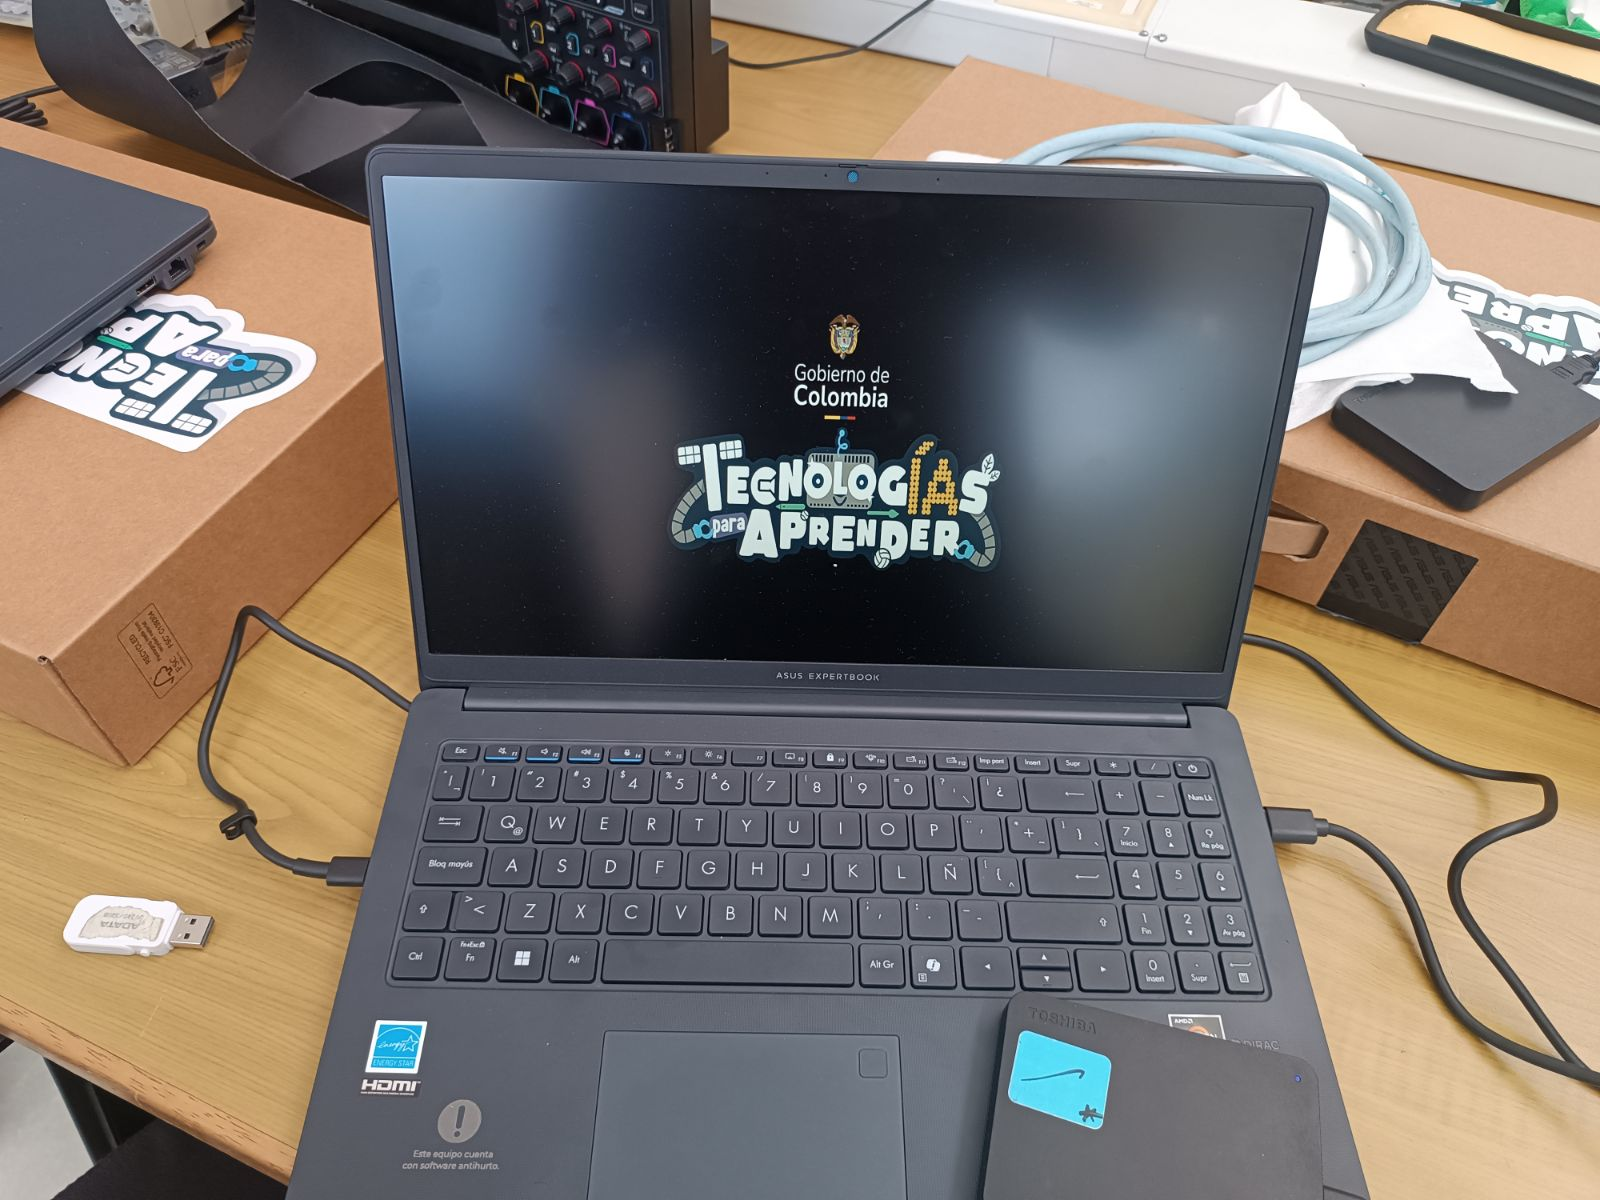
\includegraphics[width=0.8\textwidth]{Image_20261020_1306382292668009792503941.jpeg}\\[1cm]
  {\large Herramienta \texttt{ImagenMaestra.cmd} con Hiren's BootCD PE\par}
  \vspace{0.3cm}
  {\large Equipo de referencia: ASUS ExpertBook\par}
  \vfill
  {\large Repositorio \texttt{Imagenes\_Maestras\_CPE}\par}
  \vspace{0.2cm}
  {\large Octubre de 2026\par}
\end{titlepage}

\tableofcontents
\clearpage

% =====================================================================
\chapter{Introducción}
% =====================================================================

Este manual explica, paso a paso y con fotografías del proceso real, cómo se
creó una \textbf{imagen maestra de Windows} en un equipo de referencia
ASUS ExpertBook y cómo se desplegó después en un equipo de destino. Todo el
proceso se hace con un único script, \texttt{ImagenMaestra.cmd}, que abre una
interfaz con tres pestañas, una por fase.

\begin{table}[H]
  \centering
  \small
  \rowcolors{2}{grisclaro}{white}
  \begin{tabularx}{\textwidth}{@{}l l l >{\raggedright\arraybackslash}X@{}}
    \toprule
    \textbf{Fase} & \textbf{Pestaña} & \textbf{Dónde se ejecuta} & \textbf{Resultado} \\
    \midrule
    1. Preparación & Preparar y Sysprep & Windows del equipo de referencia &
      Equipo limpio, en español (es-MX), con una sola cuenta, apagado por Sysprep \\
    2. Captura & Capturar imagen & Hiren's BootCD PE, equipo de referencia &
      Archivo \texttt{Imagenes\bs Asus\_\allowbreak Imagen\_\allowbreak maestra.wim} en el disco externo \\
    3. Despliegue & Desplegar imagen & Hiren's BootCD PE, equipo de destino &
      Equipo con Windows, programas y particiones de la imagen \\
    \bottomrule
  \end{tabularx}
  \caption{Fases del proceso.}
\end{table}

\section{Materiales utilizados}

\begin{table}[H]
  \centering
  \small
  \rowcolors{2}{grisclaro}{white}
  \begin{tabularx}{\textwidth}{@{}l X@{}}
    \toprule
    \textbf{Elemento} & \textbf{Detalle} \\
    \midrule
    Equipo de referencia & ASUS ExpertBook, AMD Ryzen 5 7535HS, 16 GB de RAM,
      SSD NVMe Samsung de 1 TB, firmware UEFI \\
    USB de arranque & Memoria ADATA de 32 GB con Hiren's BootCD PE (Windows 11 PE x64),
      etiqueta \texttt{HBCD\_PE\_x64} \\
    Disco externo & Toshiba de 1 TB (931 GB útiles), NTFS, USB 3.0 \\
    Herramienta & Carpeta \texttt{IMG3\_V3} (copia del repositorio) en la raíz del disco externo \\
    Licencias & Una licencia de Windows por cada equipo de destino \\
    \bottomrule
  \end{tabularx}
  \caption{Hardware y software empleados.}
\end{table}

\foto[0.8\textwidth]{1000214233.jpeg}
  {Montaje de trabajo: equipo de referencia con la memoria USB de Hiren's
   (izquierda) y el disco externo Toshiba (derecha) conectados.}
  {fig:montaje}

\begin{importante}
El despliegue \textbf{borra por completo} el disco de destino. Antes de
confirmar, revise siempre el número, modelo y tamaño del disco seleccionado.
\end{importante}

% =====================================================================
\chapter{Obtención de la herramienta}
% =====================================================================

\section{Descargar el repositorio}

\begin{enumerate}
  \item Abra el repositorio \texttt{Imagenes\_Maestras\_CPE} en GitHub y pulse
        el botón verde \boton{Code} (figura~\ref{fig:github}).
  \item En el menú que aparece, copie la dirección HTTPS para clonarlo con Git,
        o elija \boton{Download ZIP} para descargarlo como archivo comprimido
        (figura~\ref{fig:clonar}).
\end{enumerate}

\foto{image(1).png}
  {Página del repositorio en GitHub. El botón \textsf{Code} está marcado en rojo.}
  {fig:github}

\foto{image(2).png}
  {Menú \textsf{Code}: copiar la URL HTTPS o descargar el ZIP.}
  {fig:clonar}

\section{Copiar la carpeta al disco externo}

Copie la carpeta completa a la \textbf{raíz} del disco externo. En este caso se
llamó \texttt{IMG3\_V3} (figura~\ref{fig:carpeta}).

\foto[0.7\textwidth]{image(3).png}
  {Contenido de la carpeta en el disco externo. \texttt{ImagenMaestra.cmd} es
   el script que se usa en las tres fases.}
  {fig:carpeta}

\begin{table}[H]
  \centering
  \small
  \rowcolors{2}{grisclaro}{white}
  \begin{tabularx}{\textwidth}{@{}l X@{}}
    \toprule
    \textbf{Carpeta o archivo} & \textbf{Para qué sirve} \\
    \midrule
    \texttt{ImagenMaestra.cmd} & Preparar, capturar y desplegar \\
    \texttt{CuentasCPE.cmd} & Verificar cada equipo ya desplegado \\
    \texttt{Imagenes\bs} & Aquí se guardan los archivos \texttt{.wim} capturados \\
    \texttt{Drivers\bs} & (Opcional) drivers \texttt{.inf} que se inyectan al desplegar \\
    \texttt{Respuesta\bs} & (Opcional) un \texttt{unattend.xml} propio \\
    \texttt{Logs\bs} & Registros de DISM y de cada proceso \\
    \bottomrule
  \end{tabularx}
  \caption{Estructura de la carpeta de trabajo.}
\end{table}

% =====================================================================
\chapter{Fase 1: preparación del equipo de referencia}
% =====================================================================

Esta fase se ejecuta en el \textbf{Windows del equipo de referencia}, después
de instalar y personalizar todos los programas y contenidos que llevará la
imagen.

\section{Antes de empezar}

\begin{itemize}
  \item Deje el equipo personalizado: programas, contenidos educativos, fondo
        de pantalla y accesos directos.
  \item \textbf{Desconecte internet}, para que la Microsoft Store no actualice
        aplicaciones y bloquee Sysprep. La única excepción es cuando falta el
        idioma es-MX: esa vez sí se necesita internet para descargarlo.
  \item Conecte el disco externo.
\end{itemize}

\section{Elegir las opciones}

\begin{enumerate}
  \item En el disco externo, haga doble clic en \texttt{ImagenMaestra.cmd} y
        concédale los permisos de administrador que solicita al abrirse.
  \item Vaya a la pestaña \boton{1. Preparar y Sysprep}.
  \item Marque las opciones señaladas con flechas en la figura~\ref{fig:prep-opciones}:
    \begin{itemize}
      \item \emph{Quitar automáticamente las apps de la Store que bloquean Sysprep.}
      \item \emph{Dejar SOLO la cuenta AdministradorCPE}, con la casilla
            \emph{Sin contraseña}.
      \item \emph{Equipos desplegados sin configuración inicial (directo al inicio de sesión).}
    \end{itemize}
  \item Pulse \boton{Preparar y ejecutar Sysprep}.
\end{enumerate}

\foto{image(4).png}
  {Pestaña \textsf{Preparar y Sysprep} con las opciones usadas (flechas rojas).}
  {fig:prep-opciones}

\begin{enumerate}[resume]
  \item Lea el resumen de confirmación. Indica que la cuenta AdministradorCPE
        quedará sin contraseña, qué cuentas se eliminarán con sus perfiles
        (aquí \emph{Estudiante} y \emph{Estudiantes}) y que el equipo se
        apagará al terminar. Pulse \boton{Sí} (figura~\ref{fig:prep-confirmar}).
\end{enumerate}

\foto{image(5).png}
  {Confirmación antes de ejecutar la preparación.}
  {fig:prep-confirmar}

\section{Comprobaciones automáticas}

El script revisa el equipo antes de tocar nada. En la consola inferior se ve
cada comprobación con \texttt{[OK]}, \texttt{[!]} (aviso) o \texttt{[X]} (error):

\begin{enumerate}
  \item Que el equipo no esté unido a un dominio.
  \item Que la unidad \texttt{C:} no esté cifrada con BitLocker.
  \item Que no haya reinicios pendientes.
  \item Que el almacenamiento reservado esté desactivado.
  \item Que el idioma de la imagen sea español latinoamericano (es-MX).
\end{enumerate}

\foto{image(6).png}
  {Inicio de las comprobaciones: dominio y BitLocker.}
  {fig:prep-comprobaciones}

\section{Ajuste del idioma (es-MX)}

La imagen siempre queda con \textbf{es-MX como único idioma}. Si el equipo no
lo tiene, la primera ejecución lo descarga, lo fija como idioma de pantalla y
termina con el mensaje \texttt{Preparar terminó con errores (código 1)}. No es
una falla: pide reiniciar para aplicar el idioma (figura~\ref{fig:prep-idioma1}).

\foto{image(7).png}
  {Primera ejecución: es-MX instalado y fijado. Se pide reiniciar, iniciar
   sesión con la misma cuenta, desconectar internet y volver a ejecutar.}
  {fig:prep-idioma1}

En este equipo también faltaba el español de España (es-ES), que Windows usa
como idioma de reserva de es-MX. El script lo descargó e instaló y volvió a
pedir reinicio (figura~\ref{fig:prep-idioma2}).

\dosfotos{image(9).png}{Descarga de es-ES como reserva de es-MX.}
         {image(10).png}{es-ES instalado; se pide reiniciar de nuevo.}
         {Instalación del idioma de reserva.}{fig:prep-idioma2}

\begin{nota}[Qué hacer cuando pide reiniciar]
\begin{enumerate}
  \item Reinicie el equipo.
  \item Inicie sesión con la \textbf{misma cuenta}.
  \item Desconecte internet.
  \item Abra otra vez \texttt{ImagenMaestra.cmd} y repita la pestaña
        \boton{Preparar y Sysprep} con las mismas opciones.
\end{enumerate}
Repita hasta que la comprobación de idioma salga en verde.
\end{nota}

En la siguiente ejecución la comprobación de idioma sale correcta:
\texttt{La imagen queda en es-MX como único idioma}. Después el script busca y
quita las aplicaciones de la Store que bloquean Sysprep
(figura~\ref{fig:prep-idioma-ok}).

\foto{image(8).png}
  {Idioma correcto. El proceso continúa con las apps de la Store.}
  {fig:prep-idioma-ok}

\section{Limpieza y Sysprep}

Con todo en orden, el script:

\begin{enumerate}
  \item Hace la limpieza básica de archivos temporales.
  \item Crea el archivo \texttt{C:\bs Windows\bs System32\bs Sysprep\bs unattend.xml},
        que omite la configuración inicial con idioma es-MX, teclado latinoamericano
        y zona horaria de México.
  \item Ejecuta:\\[2pt]
        \texttt{\small sysprep.exe /generalize /oobe /shutdown /quiet /unattend:C:\bs Windows\bs System32\bs Sysprep\bs unattend.xml}
\end{enumerate}

\foto{image(11).png}
  {Sysprep en ejecución (fase de limpieza de complementos).}
  {fig:sysprep}

\begin{importante}[Al terminar Sysprep]
El equipo se \textbf{apaga solo}. \textbf{No lo encienda en Windows}: si
arranca Windows, Sysprep se consume y hay que preparar de nuevo. El siguiente
arranque debe ser desde la memoria USB de Hiren's.
\end{importante}

% =====================================================================
\chapter{Fase 2: captura de la imagen}
% =====================================================================

Esta fase se ejecuta en el \textbf{mismo equipo de referencia}, arrancando
desde la memoria USB de Hiren's BootCD PE.

\section{Arrancar desde la memoria USB}

\begin{enumerate}
  \item Con el equipo apagado, conecte la memoria USB de Hiren's y el disco
        externo (figura~\ref{fig:montaje}).
  \item Encienda el equipo y entre a la utilidad de BIOS de ASUS
        (\tecla{F2} al encender). En \emph{Prioridad de arranque} debe aparecer
        la memoria USB como \emph{UEFI: Generic Flash Disk 8.07}
        (figura~\ref{fig:bios}).
  \item Pulse \tecla{F8} (\emph{Menú Arranque}) y elija
        \textbf{UEFI: Generic Flash Disk 8.07, Partition 1}
        (figura~\ref{fig:menu-arranque}).
\end{enumerate}

\dosfotos{1000214234.jpeg}{Vista general del equipo en la BIOS.}
         {1000214235.jpeg}{Detalle: SSD Samsung de 1 TB y orden de arranque.}
         {Utilidad de BIOS de ASUS (modo EZ).}{fig:bios}

\foto[0.8\textwidth]{1000214236.jpeg}
  {Menú de arranque (\textsf{F8}): se elige la memoria USB.}
  {fig:menu-arranque}

\begin{enumerate}[resume]
  \item Espere a que carguen los archivos y aparezca el escritorio de
        Hiren's BootCD PE (figura~\ref{fig:hirens}).
\end{enumerate}

\dosfotos{1000214237.jpeg}{Carga de Hiren's (\textit{Loading files}).}
         {1000214238.jpeg}{Escritorio de Hiren's BootCD PE Windows 11.}
         {Arranque de Hiren's BootCD PE.}{fig:hirens}

\section{Abrir la herramienta desde el disco externo}

\begin{enumerate}
  \item Abra \emph{This PC}. Identifique el disco externo por su tamaño: aquí
        es \textbf{Local Disk (G:)}, de 931 GB y conectado por USB 3.0
        (figura~\ref{fig:thispc}).
  \item Entre a la carpeta \texttt{IMG3\_V3} y ejecute \texttt{ImagenMaestra.cmd}
        (figura~\ref{fig:carpeta-hirens}).
\end{enumerate}

\foto[0.8\textwidth]{1000214239.jpeg}
  {Unidades vistas desde Hiren's. El disco externo es \texttt{G:}.}
  {fig:thispc}

\begin{nota}[Las letras de unidad cambian]
En Windows el disco externo era \texttt{F:}; en Hiren's pasó a ser \texttt{G:}.
La herramienta detecta su propia carpeta, así que no hay que ajustar nada.
\end{nota}

\dosfotos{1000214243.jpeg}{Carpeta \texttt{IMG3\_V3} en la raíz de \texttt{G:}.}
         {1000214244.jpeg}{Script \texttt{ImagenMaestra.cmd}.}
         {Ubicación de la herramienta en el disco externo.}{fig:carpeta-hirens}

\section{Configurar la captura}

\begin{enumerate}
  \item En la ventana, vaya a la pestaña \boton{2. Capturar imagen}.
  \item En la tabla debe aparecer la partición de Windows, \texttt{C:}
        (351,7 GB), con la columna \textbf{Sysprep = Sí}. Esto confirma que la
        fase 1 terminó bien (figura~\ref{fig:captura-pestana}).
  \item Deje marcada la casilla \emph{Añadir las particiones de recovery y datos
        del disco (PARTICION\_n)}.
\end{enumerate}

\foto{1000214245.jpeg}
  {Pestaña \textsf{Capturar imagen} con los valores iniciales.}
  {fig:captura-pestana}

\begin{enumerate}[resume]
  \item Pulse \boton{Revisar particiones} para ver qué se hará con cada
        partición antes de capturar (figura~\ref{fig:revisar}).
\end{enumerate}

\foto{1000214246.jpeg}
  {Resultado de \textsf{Revisar particiones}.}
  {fig:revisar}

\begin{table}[H]
  \centering
  \small
  \rowcolors{2}{grisclaro}{white}
  \begin{tabularx}{\textwidth}{@{}c l r X@{}}
    \toprule
    \textbf{N.\textordmasculine} & \textbf{Partición} & \textbf{Tamaño} & \textbf{Qué se hace} \\
    \midrule
    1 & EFI de arranque & 0,3 GB & No se captura; el despliegue crea una nueva \\
    2 & Reservada MSR & 0,0 GB & No se captura; el despliegue crea una nueva \\
    3 & Windows (\texttt{C:}) & 351,0 GB & Índice principal de la imagen \\
    4 & Recuperación (WinRE) & 1,5 GB & Se captura \\
    5 & Datos ``Datos'' & 300,1 GB & Se captura (30,7 GB usados) \\
    6 & Datos ``Recovery'' & 300,1 GB & Se captura (102,1 GB usados) \\
    7 & Recuperación ``MYASUS'' (FAT32) & 0,3 GB & Se captura (0,1 GB usados) \\
    \bottomrule
  \end{tabularx}
  \caption{Particiones del disco del equipo de referencia. Se capturan 4
           particiones extra en el mismo archivo \texttt{.wim}.}
\end{table}

\begin{enumerate}[resume]
  \item En \textbf{Nombre} escriba un nombre que identifique el modelo; en este
        caso escribimos \texttt{Asus\_Imagen\_maestra}. En \textbf{Descripción},
        \emph{Imagen maestra}. La línea \emph{Se guardará en} muestra la ruta
        final:
        \texttt{G:\bs IMG3\_V3\bs Imagenes\bs Asus\_Imagen\_maestra.wim}
        (figura~\ref{fig:nombre}).
\end{enumerate}

\foto{1000214247.jpeg}
  {Nombre y descripción de la imagen.}
  {fig:nombre}

\section{Ejecutar la captura}

\begin{enumerate}
  \item Pulse \boton{Capturar imagen}.
  \item Revise origen (\texttt{C:\bs}) y destino, y pulse \boton{Yes} para
        iniciar (figura~\ref{fig:captura-confirmar}).
\end{enumerate}

\foto{1000214248.jpeg}
  {Confirmación de la captura.}
  {fig:captura-confirmar}

\begin{enumerate}[resume]
  \item Espere. La captura tarda entre \textbf{20 y 60 minutos}. La barra
        inferior muestra el porcentaje y el registro se guarda en
        \texttt{G:\bs IMG3\_V3\bs Logs\bs captura\_Asus\_Imagen\_maestra.log}
        (figura~\ref{fig:capturando}).
\end{enumerate}

\dosfotos{1000214249.jpeg}{Inicio: origen, destino y archivo de registro.}
         {1000214254.jpeg}{Guardando la imagen (18\,\%).}
         {Captura en curso.}{fig:capturando}

\begin{enumerate}[resume]
  \item Al terminar aparece \emph{Imagen capturada correctamente en
        G:\bs IMG3\_V3\bs Imagenes} y en la consola \texttt{CAPTURA TERMINADA}.
        Pulse \boton{OK} (figura~\ref{fig:captura-ok}).
\end{enumerate}

\foto{IMG-20261020-WA0005.jpeg}
  {Captura terminada correctamente. En la consola se ven los índices
   \texttt{PARTICION\_3} y \texttt{PARTICION\_4} añadidos al \texttt{.wim}.}
  {fig:captura-ok}

\begin{resultado}
El archivo \texttt{Asus\_Imagen\_maestra.wim} (124,2 GB) queda en la carpeta
\texttt{Imagenes} del disco externo. El índice 1 es Windows y los índices
siguientes (\texttt{PARTICION\_1} a \texttt{PARTICION\_4}) son las particiones de
recuperación y datos.
\end{resultado}

% =====================================================================
\chapter{Fase 3: despliegue de la imagen}
% =====================================================================

Esta fase se repite en \textbf{cada equipo de destino}, también desde
Hiren's BootCD PE.

\section{Arrancar el equipo de destino}

\begin{enumerate}
  \item Conecte la memoria USB de Hiren's y el disco externo al equipo de
        destino.
  \item Arranque desde la memoria USB igual que en la captura (\tecla{F8},
        \emph{UEFI: Generic Flash Disk}). Vea las figuras~\ref{fig:menu-arranque}
        y~\ref{fig:hirens}.
  \item Abra \texttt{ImagenMaestra.cmd} desde la carpeta \texttt{IMG3\_V3} del
        disco externo.
\end{enumerate}

\section{Elegir imagen y disco de destino}

\begin{enumerate}
  \item Vaya a la pestaña \boton{3. Desplegar imagen}.
  \item En \textbf{Imagen} elija \texttt{Asus\_Imagen\_maestra.wim (124,2 GB)}
        y en \textbf{Índice} \texttt{1 - Asus\_Imagen\_maestra}.
  \item Compruebe a la derecha:
    \begin{itemize}
      \item \textbf{Firmware}: UEFI (detectado).
      \item \textbf{Respuesta\bs unattend.xml}: no (se usa el que creó la fase 1).
    \end{itemize}
  \item En \textbf{Disco de DESTINO} elija el disco interno. La columna
        \emph{Nota} indica si la imagen cabe:
\end{enumerate}

\begin{table}[H]
  \centering
  \small
  \rowcolors{2}{grisclaro}{white}
  \begin{tabularx}{\textwidth}{@{}c l r l X@{}}
    \toprule
    \textbf{Disco} & \textbf{Modelo} & \textbf{Tamaño} & \textbf{Interfaz} & \textbf{Nota} \\
    \midrule
    0 & Samsung MZVMA1T0HCLD-00BTW & 953,9 GB & SCSI & \textcolor{verdeok}{Cabe} $\leftarrow$ destino \\
    1 & Toshiba External USB & 931,5 GB & USB & Contiene las imágenes \\
    2 & Generic Flash Disk USB & 29,0 GB & USB & Pequeño: faltan 248,9 GB \\
    \bottomrule
  \end{tabularx}
  \caption{Discos detectados. La imagen necesita un disco mínimo de 717,7 GB.}
\end{table}

\begin{enumerate}[resume]
  \item Pulse \boton{Desplegar imagen}.
  \item Aparece \emph{Confirmar borrado del disco}, con el modelo y el tamaño
        del disco que se va a borrar. Si es el correcto, escriba
        \texttt{BORRAR} y pulse \boton{Borrar y desplegar}
        (figura~\ref{fig:borrar}).
\end{enumerate}

\foto{IMG-20261020-WA0009.jpeg}
  {Confirmación del borrado del disco 0 (Samsung, 953,9 GB). Se recrearán 4
   particiones de recuperación y datos.}
  {fig:borrar}

\begin{importante}
Verifique que el disco elegido \textbf{no} sea el disco externo ni la memoria
USB. La acción no se puede deshacer.
\end{importante}

\section{Proceso automático}

Después de confirmar, el script hace todo sin intervención:

\begin{enumerate}
  \item Particiona el disco según el firmware (UEFI: EFI + MSR + Windows).
  \item Aplica la imagen de Windows (índice 1).
  \item Inyecta los drivers de la carpeta \texttt{Drivers} (si hay).
  \item Copia \texttt{Respuesta\bs unattend.xml} (si existe).
  \item Crea el arranque con \texttt{bcdboot}.
  \item Recrea después de Windows las particiones de recuperación y datos
        (índices \texttt{PARTICION\_n}), con su tipo y atributos, y registra el
        entorno de recuperación (WinRE).
\end{enumerate}

Al terminar aparece \emph{Despliegue terminado. Retira el USB y el disco
externo antes de que arranque Windows. ¿Reiniciar ahora?}

\foto{1000214388.jpeg}
  {Despliegue terminado. Se restauraron las particiones de los índices 3, 4 y 5.}
  {fig:despliegue-ok}

\begin{enumerate}[resume]
  \item Pulse \boton{Yes} para reiniciar y \textbf{retire la memoria USB y el
        disco externo}.
\end{enumerate}

\section{Primer arranque del equipo desplegado}

En el primer arranque Windows termina de configurar el hardware. Aparece el
logotipo de arranque personalizado y el mensaje \emph{Preparando dispositivos}
(figura~\ref{fig:primer-arranque}).

\dosfotos{Image_20261020_1306382292668009792503941.jpeg}{Logotipo de arranque.}
         {Image_20261020_1306535857060814094690796.jpeg}{\textit{Preparando dispositivos 20\,\%}.}
         {Primer arranque tras el despliegue.}{fig:primer-arranque}

\foto[0.75\textwidth]{1000214389.jpeg}
  {Carga de Windows 11.}
  {fig:logo-windows}

En este despliegue Windows mostró la pantalla de configuración inicial para
crear el usuario:

\begin{enumerate}
  \item En \emph{¿Quién usará este dispositivo?} escriba el nombre del usuario
        (en este caso, \texttt{Estudiante}) y pulse \boton{Siguiente}
        (figura~\ref{fig:oobe-usuario}).
  \item En \emph{Crear una contraseña muy fácil de recordar} deje el campo vacío
        para que la cuenta quede sin contraseña y pulse \boton{Siguiente}
        (figura~\ref{fig:oobe-clave}).
\end{enumerate}

\dosfotos{1000214390.jpeg}{Nombre del usuario.}
         {1000214391.jpeg}{Pulsar \textsf{Siguiente}.}
         {Creación de la cuenta local.}{fig:oobe-usuario}

\foto[0.75\textwidth]{1000214392.jpeg}
  {Pantalla de contraseña.}
  {fig:oobe-clave}

\begin{enumerate}[resume]
  \item Espere mientras Windows prepara la sesión: \emph{Hola},
        \emph{Lo estamos preparando todo}, \emph{Esto podría tardar algunos
        minutos} y \emph{Ya casi está}. No apague el equipo.
\end{enumerate}

\begin{enumerate}[resume]
  \item Aparece el escritorio con la personalización de la imagen: fondo
        \emph{Computadores para Educar}, accesos directos a los programas
        educativos (Arduino IDE, Audacity, Google Chrome, entre otros) y la
        ventana \emph{Contenidos Educativos CPE} (figura~\ref{fig:escritorio}).
\end{enumerate}

\foto{1000214397.jpeg}
  {Escritorio del equipo desplegado, con la sesión \emph{Estudiante}.}
  {fig:escritorio}

% =====================================================================
\chapter{Verificación del equipo desplegado}
% =====================================================================

Después del despliegue se comprobó que las particiones y el entorno de
recuperación quedaron igual que en el equipo de referencia.

\section{Particiones}

Abra \emph{Administración de discos} (clic derecho en Inicio $\rightarrow$
\emph{Administración de discos}). El disco 0 debe mostrar las mismas
particiones que el equipo de referencia (figura~\ref{fig:discos}).

\foto{1000214427.jpeg}
  {Administración de discos en el equipo desplegado. El disco 1 es el disco
   externo, conectado para la revisión.}
  {fig:discos}

\begin{table}[H]
  \centering
  \small
  \rowcolors{2}{grisclaro}{white}
  \begin{tabularx}{\textwidth}{@{}l r l X@{}}
    \toprule
    \textbf{Partición} & \textbf{Tamaño} & \textbf{Sistema} & \textbf{Estado} \\
    \midrule
    EFI (sistema) & 300 MB & FAT32 & Creada por el despliegue \\
    Windows (\texttt{C:}) & 351,64 GB & NTFS & Arranque, archivo de paginación \\
    Recuperación (WinRE) & 1,46 GB & NTFS & Restaurada \\
    Datos (\texttt{D:}) & 300,08 GB & NTFS & Restaurada \\
    Recovery (\texttt{E:}) & 300,08 GB & NTFS & Restaurada \\
    MYASUS (\texttt{F:}) & 272 MB & FAT32 & Restaurada \\
    \bottomrule
  \end{tabularx}
  \caption{Particiones del disco 0 después del despliegue.}
\end{table}

\section{Entorno de recuperación (WinRE)}

\begin{enumerate}
  \item En la búsqueda de Windows escriba \texttt{recuperación} y abra
        \emph{Opciones de recuperación} (figura~\ref{fig:buscar-recuperacion}).
  \item En \emph{Sistema $\rightarrow$ Recuperación}, junto a
        \emph{Arranque avanzado}, pulse \boton{Reiniciar ahora} y confirme
        (figura~\ref{fig:recuperacion}).
\end{enumerate}

\foto{1000214428.jpeg}
  {Búsqueda de las opciones de recuperación.}
  {fig:buscar-recuperacion}

\dosfotos{1000214429.jpeg}{\textit{Sistema} $\rightarrow$ \textit{Recuperación}.}
         {1000214430.jpeg}{Confirmar el reinicio.}
         {Arranque avanzado desde Configuración.}{fig:recuperacion}

\begin{enumerate}[resume]
  \item El equipo reinicia en WinRE. En \emph{Choose an option} elija
        \boton{Troubleshoot} (figura~\ref{fig:winre1}).
  \item En \emph{Troubleshoot} deben aparecer \emph{Reset this PC},
        \emph{MyASUS in WinRE} y \emph{Advanced options}. Entre a
        \boton{Advanced options} (figura~\ref{fig:winre2}).
\end{enumerate}

\foto[0.75\textwidth]{1000214433.jpeg}
  {Pantalla \textit{Choose an option} del entorno de recuperación: se
   selecciona \textit{Troubleshoot}.}
  {fig:winre1}

\dosfotos{1000214434.jpeg}{\textit{Troubleshoot}, con la herramienta MyASUS.}
         {1000214435.jpeg}{\textit{Advanced options}.}
         {Opciones de solución de problemas.}{fig:winre2}

\begin{enumerate}[resume]
  \item Vuelva atrás y elija \boton{Continue} para salir a Windows 11.
\end{enumerate}

\begin{resultado}
WinRE arranca y muestra las herramientas del fabricante (MyASUS in WinRE). Eso
confirma que la partición de recuperación se restauró y quedó registrada.
\end{resultado}

% =====================================================================
\chapter{Resumen rápido}
% =====================================================================

\begin{table}[H]
  \centering
  \small
  \rowcolors{2}{grisclaro}{white}
  \begin{tabularx}{\textwidth}{@{}c X l@{}}
    \toprule
    \textbf{Paso} & \textbf{Acción} & \textbf{Figura} \\
    \midrule
    1 & Copiar la carpeta de la herramienta a la raíz del disco externo & \ref{fig:carpeta} \\
    2 & En Windows, sin internet: \textsf{Preparar y Sysprep} con las opciones marcadas & \ref{fig:prep-opciones} \\
    3 & Si pide reiniciar por el idioma: reiniciar y repetir el paso 2 & \ref{fig:prep-idioma1} \\
    4 & Esperar a que Sysprep apague el equipo; \textbf{no} arrancar Windows & \ref{fig:sysprep} \\
    5 & Arrancar Hiren's desde la USB (\textsf{F8}) con el disco externo conectado & \ref{fig:menu-arranque} \\
    6 & \textsf{Capturar imagen}: revisar particiones, poner nombre y capturar & \ref{fig:nombre} \\
    7 & En cada equipo de destino: arrancar Hiren's y abrir la herramienta & \ref{fig:hirens} \\
    8 & \textsf{Desplegar imagen}: elegir imagen y disco, escribir \texttt{BORRAR} & \ref{fig:borrar} \\
    9 & Retirar USB y disco externo, reiniciar y completar el primer inicio & \ref{fig:escritorio} \\
    10 & Verificar las particiones y el entorno de recuperación (WinRE) & \ref{fig:discos} \\
    \bottomrule
  \end{tabularx}
  \caption{Lista de pasos del proceso completo.}
\end{table}

\end{document}
